%pdflatex-../thesis.tex
% vim:spell spelllang=en_us

Themis is an application for evaluation of virtual machine migrations. It is prepared to be used for availability measurements and can be easily adjusted to perform other task during migration. 

Application is modular and can be adapted for different orchestrator or to perform different task during migration. Architecture is depicted in figure \ref{img:themis-model}. Backend is responsible for measurement management and results processing. Frontend provides web interface for users. Result can be displayed directly as table or graph in browser or exported into \Ac{CSV}.

\begin{figure}[htb]
	\begin{center}
	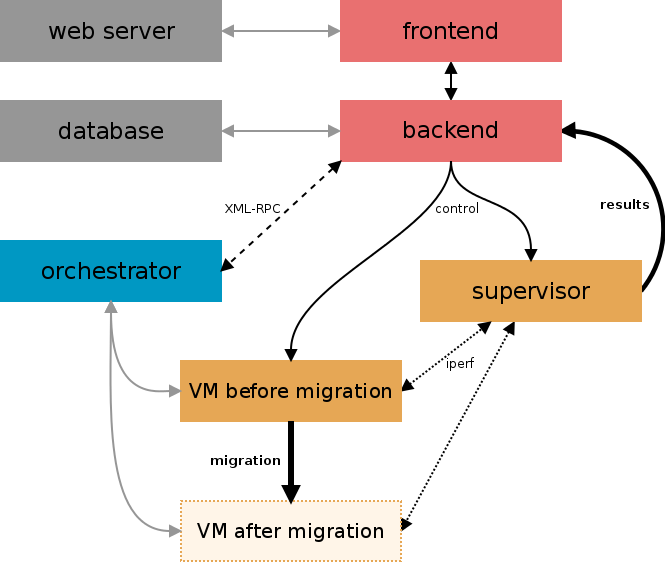
\includegraphics[width=0.7\textwidth]{themis-model.png}
	\end{center}
	\caption{Model of Themis application}
	\label{img:themis-model}

\end{figure}

% languages
Application is written in Ruby using Ruby on Rails framework. Ruby is platform independent and can run on every currently used operating system. Ruby on Rails (\Ac{RoR}) is framework providing database abstraction and strictly based on model-view-controller (\Ac{MVC}) architecture. Application is based on object model, outputs are generatied using views and controller is responsible for sending commands to models and forward results to views.

I have decided to use this framework because it provides better interaction with system services, e.g. \Ac{SSH} and \Ac{SCP}, than other web frameworks. There are public available classes for interaction with OpenNebula and OpenStack cloud \Ac{API} so it is not necessary to create \mbox{\Ac{XML}-\Ac{RPC}} parsers from scratch.

\section{Measure models}
There are three models defining measurement tasks and results. Definition, session and transfer. These models are used to describe migration tasks instructions, migration progress and results. 
Relation between models is depicted in figure \ref{img:themis-models-brief}.

All measurement models mentioned bellow are descendants of \Name{ActiveRecord::Base} and mapping between objects and tables is handled by this build-in class. It also describes inter-model associations and performs validation. 

\begin{figure}[htb]
	\begin{center}
	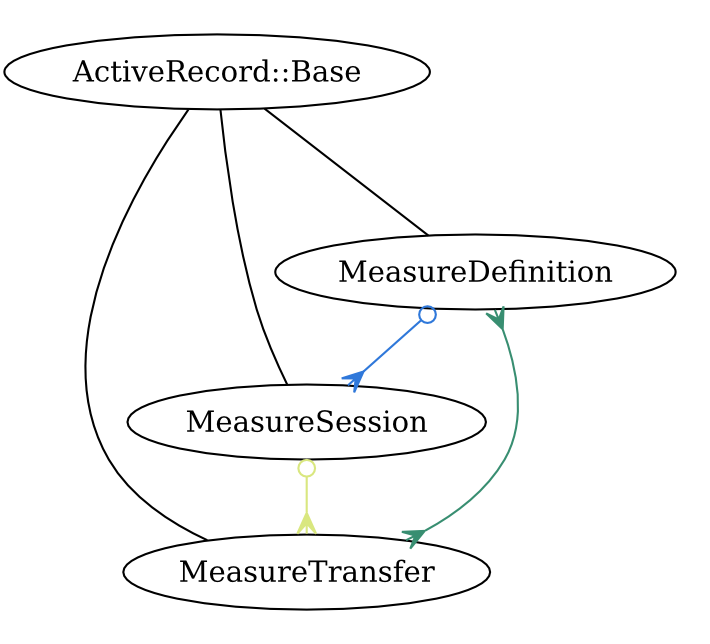
\includegraphics[width=0.6\textwidth]{models_brief.png}
	\end{center}
	\caption{Relation between measurement models}
	\label{img:themis-models-brief}
\end{figure}


\subsection{Definition}
Definition class, formally MeasureDefinition, is used to save prescription for measurement task and track time taken. Parameters are listed in table \ref{tab:measuredefinition-params} and their meaning is described bellow.

\begin{description}
	\item[vm] is virtual machine which is going to be migrated. List of \Ac{VM}s available for migration is loaded on-demand from orchestrator using OneOrchestrator class. Virtual machine must be in running state and variable \Code{THEMIS\_TYPE = 'VM'} need to be present in contextualization settings.
	\item[source] is source host for virtual machine. \Ac{VM} need to be migrated to this host before starting measurement session. List of hosts is loaded using OneOrchestrator class and hosts status is checked for each host.
	\item[destination] is destination host. \Ac{VM} is migrated to this host during measurement session.
	\item[bandwidth] is determines packet generation rate passed to agent.
	\item[cycles] set number of migration repetitions.
	\item[supervisor] is an \Ac{IP} address of supervisor services, i.e. packet receiver and result exporter
	\item[description] has an obvious meaning.

	\item[started\_at] is timestamp taken at the beginning of measurement	\item[finished\_at] is timestamp taken after finishing all migrations.
	\item[finished\_at] is timestamp taken after finishing all migrations.
\end{description}

Definition class has one-to-many relation with session class and also one-to-many indirect relation with transfer class connected through sessions. It means that is is possible to load every information from subordinate classes (models) and it is useful for generating exports and web views.

Definition class is the highest class in the hierarchy so it is connected with orchestrator. There is a class variable {@@shared\_orchestrator} which is providing link to orchestrator interface. This variable is shared by all class instances so it it not necessary to initialize more connections at once.

Methods for manipulation with orchestrator resources are declared in definition class. \Name{Host\_source} and \Name{host\_destination} returns host object for source and destination host. Method called \Name{virtual\_machine} returns virtual machine object which is going be used for migration evaluation.

Most important method of definition class is \Name{start} because it executes migration evaluation. It is responsible for generation of sessions and starting all of them. One session object will be prepared for each migration cycle, so number of session objects is same as number stored in cycles parameter. Sessions need to be started one by one so there is an loop which starts new session right after finishing of previous one. Session start is performed by calling \Name{start} of session class. This method is different from previously mentioned method with same name, because this one is defined in session class.
Finished\_at parameter is set to current timestamp right after finishing of last session, i.e. at the end of migration evaluation. 

Migration evaluation is not very computation expensive, but it can take really long time to perform many migration cycles, in particular for virtual machines under load. It is not possible to run these long running tasks on request from web interface because request will timeout shortly and task would be terminated. I have decided to use Delayed::Job (\Ac{DJ}) to run these task asynchronously.
\Ac{DJ} can run task in detached process and it can run for a long time without any timeout problems. It is also possible to run \Ac{DJ} worker on separate machine so migration evaluation is executed in completely separated environment. This approach eliminates interference with other processes or network traffic. Security is improved too, since orchestrator interface does not need to be accessible from machine with web interface.

There is one special function called flush and it clears measurement definition and all of it's subordinate objects. It can be used for debugging, because it is sometimes necessary to repeat migration with same parameters. However it is not possible to run migration which was running in the past and all of sessions have already finished.

\begin{table}[htb]
\begin{center}
	\caption{MeasureDefinition parameters}

	\label{tab:measuredefinition-params}
	\begin{tabular}{|l|l|l|l|l|}
	\hline
	\Th{Parameter} & \Th{Required} & \Th{Type} & \Th{Editable by user} & \Th{Notes} \\
	\hline
	vm & yes & string & yes & \\
	\hline
	source & yes & integer & yes & \\
	\hline
	destination & yes & integer & yes & \\
	\hline
	bandwidth & yes & integer & yes & \\
	\hline
	cycles & yes & integer & yes & required bigger than 0\\
	\hline
	supervisor & yes & string & yes & \Ac{IP} address \\ 
	\hline
	description & no & text & yes & \\
	\hline
	started\_at & no & timestamp & no & \\
	\hline
	finished\_at & no & timestamp & no & \\
	\hline
	\end{tabular}
\end{center}
\end{table}


\subsection{Session}
Session class, precisely MeasureSession, is a link between definition and transfers. This class is responsible for migration and measurement coordination. Remote management of virtual machines and orchestrator is performed inside this class.

There are no parameters editable by user because all necessary information about migration are inherited from definition. Table \ref{tab:measuresession-params} describes all parameters. There are two timestamp fields with evident purpose, reference to MeasureDefinition and two fields special for this class:
\begin{description}
	\item[seq] is sequence number in scope of superior MeasureDefinition. Session with \mbox{$\mathrm{seq} = 0$} is going to be executed first and $\mathrm{seq} = \mathrm{measure\_definition.cycles}$ is the last one.
	\item[status] determines status of measurement session:
		\begin{itemize}
			\item \B{0} - pending - session is waiting for execution, this is default state
			\item \B{1} - running - session is running right now
			\item \B{2} - done - migration was finished successfully
			\item \B{3} - failed - migration was executed and failed to finish
		\end{itemize}
\end{description}

\begin{table}[htb]
\begin{center}
	\caption{MeasureSession parameters}
	\label{tab:measuresession-params}
	\begin{tabularx}{\textwidth}{|l|l|l|l|X|}
	\hline
	\Th{Parameter} & \Th{Required} & \Th{Type} & \Th{Edit.} & \Th{Notes} \\
	\hline
	status & yes & integer & no & \\ 
	\hline
	seq & yes & integer & no & \\
	\hline
	started\_at & no & timestamp & no & \\
	\hline
	finished\_at & no & timestamp & no & \\
	\hline
	\hline
	measure\_definition\_id & yes & reference & no & reference to MeasureDefinition \\

	\hline
	\end{tabularx}
\end{center}
\end{table}


Most important part of MeasureSession class is \Name{start} method. This method is executed by superior definition, so it is not necessary set asynchronous execution with Delayed::Job, because higher object is already running asynchronously.

It is necessary to load migration parameters, so only an information about supervisor \Ac{IP} is loaded as a string and the rest is loaded as and objects. It is beneficial to work with objects instead of identifiers because it allows to execute commands directly without any additional parsing.

Net::SSH client library is used for connection to virtual machine under test and supervisor. I have implemented authentication with keys because it is necessary to provide password-less login for backend service. It is possible to implement password authentication just by editing client library configuration, but I wanted to avoid storing any password in source code. 

Migration process can be divided into 3 stages. First stage is preparation for migration, second stage is migration and third stage is migration verification and reporting. Tasks must be carried out sequentially because next task always depends on previous one.

First task after loading migration information is clearing previous measurement session. Established session between packet generator and packer receiver can become stale if it was not terminated successfully during previous migration. Packet generator and receiver should be terminated after virtual machine migration, but it may stay running in case of unexpected backend error or unclean shutdown. Command \ref{cmd:killcmd} is executed on \Ac{VM} and supervisor just to be sure there are no stale sessions. This command is optimized for agent.rb and need to be adapted to work with another measurement tools.

\begin{figure}[htb]
\caption{Clear stale sessions command}
\label{cmd:killcmd}
\begin{verbatim}
KILLPID=$(ps aux | grep -v grep | grep agent\.rb | grep ruby \
| xargs | cut -d' ' -f2); if [ -n "$KILLPID" ]; then \
kill -SIGINT "$KILLPID"; fi 
\end{verbatim}
\end{figure}

Next action performed during first stage is migration to source host. Source and destination hosts are loaded from measure definition and migration must be performed exactly from source to destination, so \Ac{VM} need to be running on source host. Unmeasured migration to source host is requested during this stage if \Ac{VM} is not already running on right host.

Last task in preparation stage is to run agents. It is necessary to start agents on \Ac{VM} and supervisor and both agents must stay running after \Ac{SSH} disconnection. It is a bit tricky to run Ruby script in remote machine in subshell, because normal behavior it is terminate process after disconnection. I am using \Cmd{screen} software which is able to run detached processes. However situation is even more complicated due to different Ruby installation methods on \Ac{VM} and supervisor. Virtual machine uses standard Ruby version installed via package manager by command \Cmd{apt-get install ruby}, so it easier to run agent.rb because it do not require interactive shell. Rbenv\footnote{\url{https://github.com/sstephenson/rbenv}} is used to install Ruby on supervisor because agent.rb in receiver mode requires newer version than provided by package manager. Rbenv is initialized in file \~/.bashrc so it is necessary to run all Ruby script in interactive shell. Parameters for agent.rb can be found below in table \ref{tab:agent-parameters}.

\begin{figure}[htb]
\caption{Run remote agents command}
\label{cmd:remote agents}
\begin{verbatim}
###  generator - VM
screen -d -m /bin/bash -c '~/themis/agent.rb "generator" \
#{supervisor} #{5000 + (id % 1000)} #{measure_definition.bandwidth}M'

### receiver - supervisor
screen -d -m /bin/bash -li -c '~/themis/agent.rb "receiver" \
#{supervisor} #{5000 + (id % 1000)} \
#{measure_transfers_upload_url(:measure_session => id, :format => 'json')}'
\end{verbatim}
\end{figure}


\cleardoublepage
	













\subsection{Transfer}

% delayed job


\section{Virtual machines}

\section{Agent}
It was necessary to develop a script wrapper capable to parse iperf output and upload results to backend module. This script is called agent.rb, it is attached on on the CD and will be published in project repository. It is written in Ruby to be compatible with rest of the project. Agent script is executed from backend in migration\_session model in start method and \Ac{SSH} is used for remote execution.

Agent script need to be available in virtual machine under test as well as in hypervisor. However distribution is fairly simple because it is just a single file (agent.rb) with a few dependencies. This file can be distributed manually, which is not very usable for large or frequent deployment. Automatic deployment using OpenNebula's contextualization is much more efficient since orchestrator takes care of saving file into \Ac{VM}s. 
It is also possible to use configuration management system to upload this file and prepare environment to run migration. I have used Ansible to deploy agent.rb because it was necessary to update Ruby version. 

There are two modes of running agent. Modes differ in packet generator parameters and required dependencies. Mode is determined by \Code{ARGV[0]} parameter, which is the first parameter after filename. It is necessary select correct mode and properly configure all parameters from table \ref{tab:agent-parameters} because measure session can not be established otherwise. 

Generator mode only generates packets and sends them to receiver so it require nothing more than Ruby and iperf available. Receiver mode is more advanced and it uploads results to backend besides receiving packet. Receiver mode requires these dependencies:
\begin{itemize}
	\item \B{net/http} is used to upload results to backend using \Ac{HTTP} POST method
	\item \B{json} is necessary to export data into \Ac{JSON} before sending
	\item \B{date} is used to parse timestamp provided iperf and convert it into backend compatible format
\end{itemize}

% dependencies 
Both modes use IO class to read pipeline output from iperf program. This class is, however, part of Ruby core so it is not necessary to install it separately. Receriver dependencies can be install using distribution package manager or with gem utility using command \Cmd{gem install net/http json date}.

\begin{table}[htb]
\begin{center}
	\caption{Agent.rb parameters}
	\label{tab:agent-parameters}
	\begin{tabularx}{\textwidth}{|r|l|l||l|X|}
	\multicolumn{3}{c}{\Th{Generator mode}} & \multicolumn{2}{c}{\Th{Receiver mode}} \\
	\hline
	\# & {Parameter} & {Example}  & {Parameter} & {Example} \\
	\hline
	\hline
	0 & Mode & generator & Mode & receiver \\
	\hline
	1 & Destination \Ac{IP} & 192.0.2.1 & Listen \Ac{IP} & 192.0.2.1 \\
	\hline
	2 & Destination port & 5004 & Listen port & 5004 \\
	\hline
	3 & Bandwidth & 1M & Upload \Ac{URL} & \url{http://backend/measure_transfers/23.json} \\
	\hline
	\end{tabularx}
\end{center}
\end{table}


% iperf crap
Agent is using legacy iperf version developed by NLANR/DAST but it introduces several problems which must be resolved in agent.rb and measure session routine. I am going to adapt agent.rb for iperf3\footnote{Available on \url{https://github.com/esnet/iperf}} which is new implementation developed by ESnet/Lawrence Berkeley National Laboratory. Iperf3 provides \Ac{JSON} output and probably will not suffer from problems presented below.

First problem is automatic session reestablishment. This occurs when running session is interrupted by a client and new session is initialized with the same receiver in short interval (less than few seconds). Iperf server joins new session with previous one which is not desired solution. This it the reason why there is 5 second interval inserted before generator restart. 

Second problem is handling INT signal by legacy iperf. SIGINT is reserved for external interrupt and this signal is for example sent to process when \mbox{Ctrl + C} is pressed. Iperf catches this signal preventing user to accidentally stop measure session. I understand reason why this function was implemented but I think that is total nonsense to require two consecutive INT signals to quit program. I have solved this by trapping SIGINT and sending KILL signal to iperf before agent.rb exit. This is only one possible way to reliably stop running agent together with iperf.

\begin{figure}[htb]
\caption{Example of agent.rb and iperf commands}
\label{code:fw}
\begin{verbatim}
# agent in generator mode
./agent.rb "generator" 192.0.2.1 5004 10M
# expanded iperf command in generator mode
iperf --udp --interval 1 --time 3600 --client 192.0.2.1 --port 5004 \
--bandwidth 10M --format b
	
# agent in receiver mode
./agent.rb "receiver" 192.0.2.1 5004 http://backend/measure_transfers/23.json
# expanded iperf command in receiver mode
iperf --server --bind 192.0.2.1 --port 5004 --udp --interval \
--reportstyle c --format
\end{verbatim}
\end{figure}


\section{Application}
	% backend
	% frontend
	% orchestrator
	% database
	% web server

	% měření pro elmag

